\section{Implementation}

The AI4Agile app was implemented within Jira Cloud as an app and connected to a Python-based backend.

\subsection{Frontend}

As part of the Atlassian Design Guidelines, a frontend library, Atlassian User Interface (AUI), is provided to create new UI elements to match Jira’s style and user experience. Needed components that were missing from the AUI were crafted by the provided Design Guidelines from Atlassian.

Within Jira, all objects (epics, stories, issues) are rendered in the same way, each containing a shared issue panel as shown in figure \ref{fig:issueView}. Our app is implemented within the issue panel in the form of additional panels that can be opened through newly introduced buttons to the primary button set. When a process button or visualization button is pressed, a new panel, built with HTML and javascript, will render and be focused on.

Each of the processes use the same suggestion panel, with variations depending on the need for user inputs in the case of epic decomposition and story optimization. The suggestion module, when opened, requests suggestions from the backend through jQuery AJAX and displays a loading animation until the suggestions are received. Stories can be changed and once checked, they can be created which is done by passing the selected stories via an AJAX call to the backend. The responsibility to populate selected stories to the Jira board is by the backend.

\begin{figure*}
\centerline{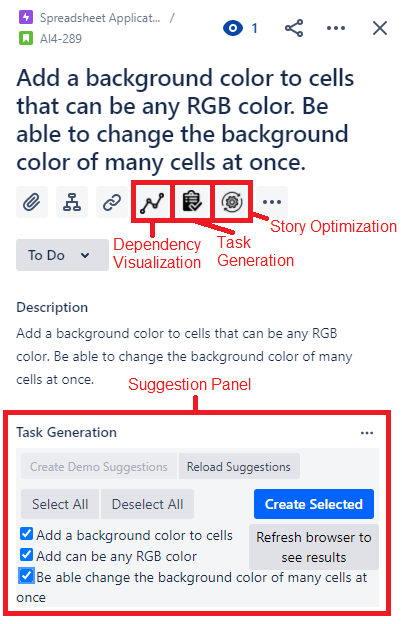
\includegraphics[width=\textwidth,height=\textheight,keepaspectratio]{./figure/Frontend.png}}
\caption{Issue View within Jira while the Task Generation process shown after suggestions are recieved}
\label{fig:issueView}
\end{figure*}

\subsection{Backend}

The backend served two primary functionalities: generating suggested issues and populating selected suggestions into Jira. Each process has its corresponding suggestion generator and selected suggestion creator since the specifics of each type of issue varies. Jira treats all issue types (i.e. epics, stories, and tasks) the same, each having the same set of shared fields with the addition of custom fields depending on the type of issue.

All three processes were implemented using Python due to the available libraries and as a result the primary interface was also implemented using Python. The interface uses Flask, a Python web framework, to receive the messages sent by AJAX in the frontend. The information needed from the issues are gathered by querying the Atlassian Rest API through an open-source Python library, “atlassian-Python-api”, which simplifies Atlassian API calls. When generating suggestions, the description is queried for and passed as a list of individual requirements to the text processor. Suggestions are then passed back through a reply to the original message. Once a user selects, and possibly edits, which issues they would like to have populated in their Jira board, then the original issue is queried again to percolate existing fields, such as assignee, reporter, due date, tags, or sprints, to the newly created child issues. Each newly created issue is given a blocking relationship to the issue they were derived from. For example, all of the created stories from an Epic Decomposition will “block” the epic from being completed. Any further tasks created from Task Generation on a story will “block” the story from completion.

\subsubsection{Epic Decomposition}
The Epic Decomposition process was implemented using k-means clustering over a dynamic clustering technique, such as DBSCAN or Mean-shift. Dynamic clustering techniques were unable to be implemented in a manner that yielded consistent meaningful clusters across many epic inputs. This was a result of an inability to filter noise such that the clusters were neither completely disjoint or entirely overlapping. Thus, k-means, a centroid-based clustering algorithm, was used at the cost of selecting a default number of stories to generate. The default number of stories generated is five but the user can select between 2 and 10 stories using a newly added slider in the UI for the Epic Decomposition process.

\subsubsection{Story Optimization}
For Story Optimization, the process maintained the initial implementation without any significant changes to the algorithm. The algorithm utilizes a pre-trained Word2Vec model, along with SIF and cosine similarity functions from the scikit-learn python library. Initially, the degree of connectivity between sentences was specified by choosing the optimal threshold level. However, it was changed so that the user can choose to increase or decrease the degree of connectivity between sentences offering more flexibility in the generated results.

The user can choose to increase or decrease the degree of connectivity between sentences. The slider displays options from 0 to 10, which maps to values from 0.65 to 0.75 as threshold values on the backend. The slider integration was a feature that was added based on mentor feedback. A parameter is exposed to give the user more control of the output. The exposed parameter is the degree of connectivity between the sentences. It was determined after impact analysis that it is better to implement it this way because it generates more meaningful results tailored to each user. This also eliminates the need for having a fixed threshold number, since the optimal threshold number can vary between inputs.

\subsubsection{Task Generation}
The approach for Task Generation was based off a decomposition approach by Das, Majumder, and Phadikar in 2018\cite{b3}. Initially the natural language toolkit (NLTK) library was selected for implementing task generation, but it lacked the need for parts-of-speech tagging. The main feature that NLTK lacked was word dependency. Word dependency is important to this process, since this was the main feature used to create simple sentences. Word dependency returns a pair of words, identifying the dependency between the two. The new Python library being used is Stanza. This library allows for parts-of-speech tagging, word dependency, and tree parsing. By having part-of-speech tagging and word dependency, the creation of simple sentences from complex and compound sentences was easier to implement.

\subsection{Communication}
\begin{figure*}
\centerline{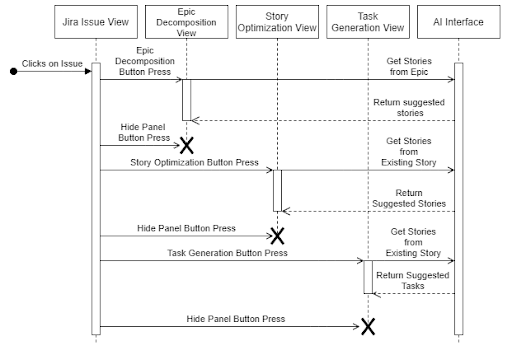
\includegraphics[width=\textwidth,height=\textheight,keepaspectratio]{./figure/SequenceFlowDiagram.png}}
\caption{Suggestion web panel sequence diagram representing the flow of messages between the frontend Jira web page and AI4Agile backend}
\end{figure*}

The plugin communicates from Jira to the backend interface via a listener through AJAX calls which are received by Flask. When a web panel is opened for any of the three processes, a message is sent to generate and return the suggestion issues. The Jira panel will function asynchronously with a loading animation appearing until the resulting suggestions are received. Once the results are received, populated in the suggestion box, and the desired suggestions are selected by the user, then a message is sent containing which suggestions to then create within Jira.

\begin{center}
\begin{table}
\caption{Components, subcomponents, and sources used for implementation of subcomponents}
\begin{tabular}{ |c|c|c| } 
\hline
\multicolumn{1}{|c|}{\textbf{Component}} & \multicolumn{1}{c|}{\textbf{Subcomponent}} & \multicolumn{1}{c|}{\textbf{Source}} \\
\hline
Epic Decomposition & K-means clustering & scikit-learn: machine learning in Python \\
\hline
\multirow{4}{*}{Story Optimization} & Word embedding & Google Word2Vec Pre-trained Model \\ 
\cline{2-3}
& Feature Extraction & scikit-learn: machine learning in Python \\ 
\cline{2-3}
& Cosine similarity & scikit-learn: machine learning in Python \\
\cline{2-3}
& Function decision &N/A \\ 
\hline
\multirow{2}{*}{Task Generation} & Sentence classification & Stanford CoreNLP \\ 
\cline{2-3}
& Part of speech tagging & Natural Language ToolKit \\ 
\hline
\multirow{3}{*}{UI} & Tree relationship graph & Cytoscape \\ 
\cline{2-3}
& Clustered relationship graph & Cytoscape \\ 
\cline{2-3}
& Jira Cloud frontend & Atlassian Connect Express Modules \\ 
\hline
\end{tabular}
\end{table}
\end{center}